%%
%% Author: clement_besnier
%% 17/05/2018
%%

\documentclass[11pt]{article}
\usepackage[utf8]{inputenc}
\usepackage[T1]{fontenc}

\usepackage[bookmarks=true]{hyperref}
\usepackage[a4paper,margin=2cm,headheight=15pt]{geometry}
\usepackage{float}
\usepackage{textcomp}
\usepackage[english]{babel}
\usepackage{listings}
\usepackage{caption}

\usepackage[ruled,vlined,linesnumbered]{algorithm2e}
\SetKwFor{Loop}{Loop}{}{EndLoop}

\usepackage{amsthm}
\usepackage{mathrsfs}
\usepackage{rotating}
\usepackage{stmaryrd}
\usepackage{wrapfig}
\usepackage{xcolor}
\usepackage{tikz}
\usepackage{fancyhdr}
\usepackage{pifont}
%\usepackage{lmodern}
\usepackage[notextcomp]{kpfonts}
\usepackage{amsmath,amsfonts,amssymb}

\graphicspath{{images/}}
%\usepackage[firstpage]{draftwatermark}
%\SetWatermarkLightness{0.8}
%\SetWatermarkAngle{25}
%\SetWatermarkScale{2.5}
%\SetWatermarkFontSize{1cm}
%\SetWatermarkText{\sc{Ne pas emporter}}

%\usepackage[
%type={CC},
%modifier={by-nc-sa},
%version={3.0},
%]{doclicense}




\title{doc kraken}
\author{Clément Besnier}
\date{May 2018}

\begin{document}
    \selectlanguage{english}
    \maketitle
    \newpage

    \begingroup
    \setcounter{footnote}{0}% Reset footnote counter
    \renewcommand{\thefootnote}{\fnsymbol{footnote}}% Modify footnote printing
   % \href{mailto:pierre-francois.gimenez@irit.fr}{pierre-francois.gimenez@irit.fr}
    %\href{mailto:clemsciences@aol.com}{clemsciences@aol.com}
  %  In French: \url{TechTheTroll.wordpress.com} % avant
   % In French: \url{clementbesnier.pythonanywhere.com}
    \endgroup

    \newpage
    \tableofcontents




    \section{Introduction}\label{sec:introduction}

    In this doc, we only considere a robot which is:
    \begin{itemize}
        \item non-holonomic, which cinematically behaves like a car
        \item with %muni de codeurs;
        \item with proximity sensors %muni de capteurs de proximité;
        \item autonomous and does not need to cooperate % qui n'a pas besoin de coopérer.
    \end{itemize}

    If you want to read only one chapter, beware the dependencies between sections
    \begin{center}
        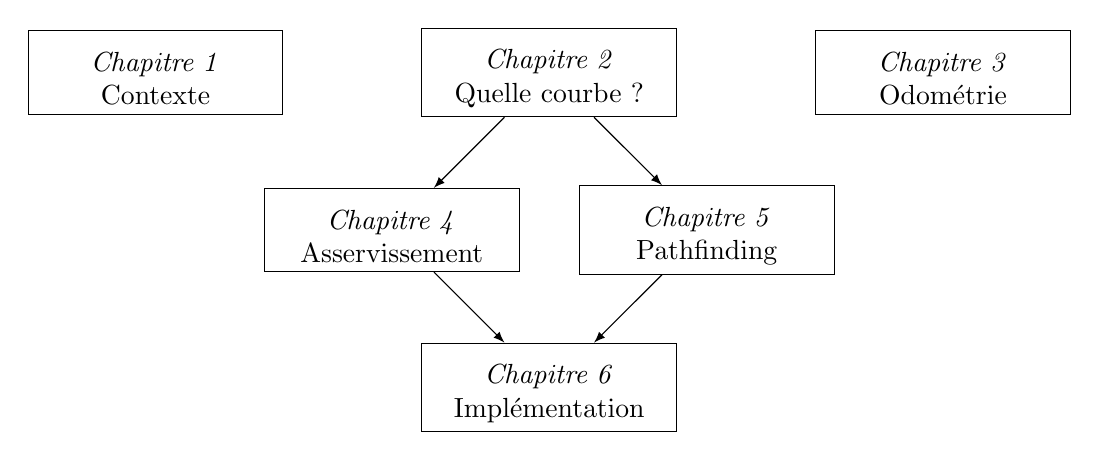
\begin{tikzpicture}[every path/.style={>=latex},every node/.style={draw,circle}]
            \node[rectangle,text width=3cm, text height=0.4cm, align=center] (1) at (0,4)  { \textit{Chapitre 1} \\ Contexte};
            \node[rectangle,text width=3cm, text height=0.4cm, align=center] (2) at (5,4)  { \textit{Chapitre 2} \\ Quelle courbe ?};
            \node[rectangle,text width=3cm, text height=0.4cm, align=center] (3) at (10,4)  { \textit{Chapitre 3} \\ Odométrie};
            \node[rectangle,text width=3cm, text height=0.4cm, align=center] (4) at (3,2)  { \textit{Chapitre 4} \\ Asservissement};
            \node[rectangle,text width=3cm, text height=0.4cm, align=center] (5) at (7,2)  { \textit{Chapitre 5} \\ Pathfinding};
            \node[rectangle,text width=3cm, text height=0.4cm, align=center] (6) at (5,0)  { \textit{Chapitre 6} \\ Implémentation};
            \draw[->] (2) edge (4);
            \draw[->] (2) edge (5);
            \draw[->] (4) edge (6);
            \draw[->] (5) edge (6);
        \end{tikzpicture}
    \end{center}


    \section{Mathematical background}\label{sec:mathematicalBackground}

    \subsection{Path}\label{subsec:path}
    The easiest way to move with a robot is to make rotations and translations.
    \subsection{Curved Path}\label{subsec:curvedPath}
    Definition:

    Criteria:
    \begin{itemize}
        \item ExpressivityLeur expressivité, c'est-à-dire à quel point les courbes du modèle pourront se rapprocher de n'importe quelle courbe;
        \item Constraints on the robot: %Les contraintes du robot en tant que système mécanique possédant une inertie, une précision limitée, … (ce qui, en terme de courbe, impose la continuité de certaines grandeurs);
        \item Math: %La difficulté mathématique. Certaines courbes sont plus difficiles à exprimer et à calculer que d'autres (faut pas oublier qu'on est sur système embarqué…).
    \end{itemize}

    \subsection{Circular arc}\label{subsec:circularArc}
    %Dans ce modèle, le robot suit une succession d'arcs de cercles et de lignes droites (qui peuvent être interprétées comme des formes dégénérées d'arc de cercles de rayon infini). Ces arcs de cercles sont enchaînés de manière à obtenir une courbe continue et dérivable (l'orientation du robot à la sortie d'un arc est la même qu'à l'entrée de l'arc suivant).

%    \begin{figure}[H]
%        \centering
%        \includegraphics[width=8cm]{arcs.png}
%        \caption{Exemple d'une succession d'arcs de cercle. L'œil voit très bien ces discontinuités.}
%    \end{figure}
%
%    Mathématiquement, il s'agit d'un modèle simple, quasiment tous les calculs qu'on souhaite faire sont réalisables facilement. Un autre avantage : on a la preuve de l'optimalité d'une telle trajectoire en terme de minimisation de distance \cite{reeds1990optimal}.
%
%    Par contre, il y a un problème : une succession d'arcs est seulement $\mathcal{C}^1$, ce qui signifie que le robot va subir des discontinuités\footnote{que ceux qui ont pensé \emph{"scontinuités"} sortent} d'accélération, résultant en un mauvais suivi de la trajectoire. En effet, si on note $\Delta R$ la différence entre les rayons de deux arcs de cercle consécutifs, un robot à vitesse $v$ et de masse $m$ va subir au changement d'arc une force centrifuge $F_c$:
%    \[F_c = \frac{m v^2}{\Delta R}\]
%    Plus le robot sera rapide, plus cette force sera grande, ce qui risquera dans le meilleur des cas de faire glisser le robot orthogonalement à son orientation (induisant une erreur sur les codeurs qui ne peuvent pas mesurer ce mouvement latéral), et dans le pire des cas de soulever voire de faire chuter le robot si son centre de gravité est trop haut.
%
%    Des mécanismes d'anticipation de trajectoires existent afin de limiter les problèmes de suivi de trajectoire, mais ces discontinuités nous ont poussé à disqualifier ces courbes.



    \subsection{Bezier Curve}\label{subsec:bezierCurve}
    \href{https://en.wikipedia.org/wiki/B\%C3\%A9zier\_curve}{https://en.wikipedia.org/wiki/B\%C3\%A9zier\_curve}
%    Ah, les courbes de Bézier ! Elles sont zolies, et en plus elles sont $\mathcal{C}^\infty$, ce qui signifie que mécaniquement il n'y aura aucune discontinuité.
%
%    Le problème est cette fois plus d'ordre mathématique : leurs expressions ne sont pas simples et il n'est pas forcément facile de planifier un chemin en cherchant des points de contrôle qui peuvent être dans des obstacles.
%
%    \begin{figure}[H]
%        \centering
%        \includegraphics[width=8cm]{Bezier_rec.png}
%        \caption{Exemple d'une courbe de Bézier et de sa construction. Les points de contrôle sont A, B, C et D. La courbe de Bézier en elle-même est en bleu.}
%    \end{figure}
%
%    Cette fois, c'est plus pour des raisons de difficultés mathématiques que nous avons mis de côté ces courbes.

    \subsection{Clothoids}\label{subsec:clothoids}
    Also called Euler spiral \href{https://en.wikipedia.org/wiki/Euler\_spiral}{https://en.wikipedia.org/wiki/Euler\_spiral}, clothoids have wonderful properties so that we use them for all our motorways and railways, where straight lines join \cite{baass1982use}, for fonts and design.
    
    Let's assume we are driving a car with a constant speed. Then we are turning the wheel. That's all, the trajectory of the car is describing a clothoid! What is great with clothoids is that the derivative of the curvature of clothoids is a constant and this is good for cars.
    
%    \begin{figure}[ht]
%        \centering
%        \includegraphics[width=8cm]{Cornu_Spiral.png}
%        \label{fig:clotho}
%        \caption{La clothoïde, c'est elle \textit{\#swag}}
%    \end{figure}

    \textbf{Remarque :} From now, $'$ means the deriation according to curvilinear abscissa $s$.

    If $\theta(s)$ is the orientation of the robot at $s$, the curvature at $s$ is :
    \[\kappa(s) = \theta'(s)\]
    The greater the absolute value of the curvature, the faster we turn.
    
    En gros, plus la valeur absolue de la courbure est grande, plus on tourne vite. De plus, si on approche la trajectoire du robot en $s$ par un cercle (appelé cercle osculateur), alors le rayon $R(s)$ de ce cercle est appelé rayon de courbure\footnote{plus précisément, c'est le rayon algébrique, qui peut être négatif} et vaut\footnote{notez, cette définition n'est pas utilisée par la suite. C'est juste que savoir que la courbure est l'inverse du rayon du courbure, dans la vie, c'est important} :
    \[R(s) = \frac{1}{\kappa(s)}\]
    Its parametric equation is:
    \begin{align*}
        \tag{*}
        p(t) = a \int_0^t e^{i u^2} \, du
        \label{equ:clotho_param}
    \end{align*}
    A clothoid is thus a curve such that $\kappa(s)' = C$.

    A unitary clothoid ($C = 1$) may be drawn thanks to its power series:
    \begin{align*}
        \tag{**}
        \begin{cases}
            x &= s - \frac{s^5}{1 \cdot 2 \cdot 5} + \frac{s^9}{1 \cdot 2 \cdot 3 \cdot 4 \cdot 9} - ... = \sum_{n=0}^{+\infty} \frac{(-1)^n \cdot s^{4n+1}}{(2n)! \cdot (4n+1)} \\
            y &= \frac{s^3}{1 \cdot 3} - \frac{s^7}{1 \cdot 2 \cdot 3 \cdot 7} + \frac{s^{11}}{1 \cdot 2 \cdot 3 \cdot 4 \cdot 5 \cdot 11} - ... = \sum_{n=0}^{+\infty} \frac{(-1)^n \cdot s^{4n+3}}{(2n+1)! \cdot (4n+3)}
        \end{cases}
        \label{equ:clotho}
    \end{align*}
    %\begin{figure*}[ht]
    %	\centering
    %	\includegraphics[width=200pt]{doge.jpg}
    %\end{figure*}

    Ces calculs de série peuvent être effectués une fois pour toutes, les clothoïdes étant toutes similaires entre elle (sauf dans le cas particulier de la ligne droite et des cercles, c'est-à-dire quand $\kappa' = 0$)

    Par contre, il y a certains calculs qui devront être approchés, notamment la distance d'un point à la courbe\footnote{on en reparlera après}.
    The distance between a point and the curve.

%    \begin{wrapfigure}[15]{r}{180pt}
%        \includegraphics[width=180pt]{doge.jpg}
%    \end{wrapfigure}
	
    De plus, si on fait intervenir la vitesse angulaire $\omega(s)$ et la vitesse instantanée $v(s)$ du robot, on a la relation suivante :
    \[\omega(s) = v(s) \times \theta'(s) = v(s) \times \kappa(s)\]
    Mais on n'est pas obligé de suivre une clothoïde à vitesse constante. Il suffit d'avoir :
    \[\kappa(s)' = \left(\frac{\omega(s)}{v(s)}\right)' = C\]
    soit\footnote{même si en pratique, rassurez-vous, on n'utilisera pas cette équation}
    \[\frac{\omega'(s) \times v(s) - v'(s) \times \omega(s)}{v(s)^2} = C\]
    Au final, les clothoïdes sont bien pratiques, mécaniquement. Nous avons donc choisi une succession d'arcs de clothoïdes comme trajectoire courbe pour ces raisons. Mathématiquement, c'est globalement facile (on verra ça en détail dans un chapitre ultérieur).

%    \begin{figure}[ht]
%        \centering
%        \includegraphics[width=10cm]{traj.png}
%        \caption{Exemple d'une succession de clothoïdes. L'arc de cercle et la ligne droite en sont des cas particuliers. En bas, la courbure : elle est continue.}
%    \end{figure}
%
%    Finalement, la conclusion à ce chapitre revient à l'article \cite{bertolazzi2012fast} : \emph{"It is well known that the best or most pleasing curve is the clothoid, despite its transcendental form".}
%
%    \begin{figure}[ht]
%        \centering
%        \includegraphics[width=5cm]{clothoid_loop.jpg}
%        \caption{La clothoïde ménage les moteurs comme les cœurs. Ici, deux clothoïdes sont raccordées.}
%    \end{figure}
%
%    \begin{figure}[ht]
%        \centering
%        \includegraphics[width=6cm]{spiro1.png}
%        \caption{Utilisation en design.}
%    \end{figure}


    \section{}

     \href{https://en.wikipedia.org/wiki/Rotary\_encoder}{https://en.wikipedia.org/wiki/Rotary\_encoder}


    On appelle \emph{codeur} un capteur rotatif qui permet de connaître les déplacements du robot. Il y en a deux, un pour chaque roue de propulsion. Ils sont soit intégrés aux moteurs, soit montés sur des roues folles. Ce deuxième cas, un peu plus lourd à mettre en œuvre mécaniquement, à l'avantage de détecter les patinages (quand les roues tournent mais glissent, ce qui fait que le robot ne bouge pas).

    A partir des informations provenant de ces codeurs, on peut estimer la position du robot.

    Il y a plusieurs moyens d'approcher la position du robot à partir du mouvement des codeurs en utilisant des approximations. On peut voir deux principales approximations.

    \subsection{Linear Approximation}\label{subsec:linearApproximation}

    On suppose que le robot suit des lignes brisées. C'est un calcul simple à mettre en place qui suffit le plus souvent… sauf en cas de trajectoire courbe.

    \subsection{Circular Approximation}\label{subsec:circularApproximation}

    Une approximation plus complexe (dont le cas linéaire est un cas particulier) mais qui est bien plus adaptée aux trajectoires courbes. En plus, c'est une approximation qui fait naturellement intervenir le calcul de la courbure que suit le robot ; et sans trop vouloir \textit{spoiler}, ça nous sera utile.

    Le lecteur intéressé est invité à lire le document de l'équipe RCVA sur le sujet\cite{odorcva}\footnote{\url{http://www.rcva.fr/images/stories/site/cours/Odometrie2010/ODOMETRIE\_2010.pdf}}. Il est complet et je n'ai rien à y ajouter.



    \section{Pathfinding}\label{sec:pathfinding}
	Here is presented the core of this docs: finding the shortest path between a start point to a goal point. To begin with, let's introduce an abstract definition of our aim: Let a weighted graph G = (E,V), with E the set of edges and V the set of vertices (or nodes), and a function $\delta$, such that $\delta(e) \in \Re_{+}$. V represents the possible positions of the robot, E the possible paths between positions and $\delta$ the cost of an edge (because moving costs time!). 
	The start node is $n_S \in E$ and the goal node $n_G \in E$.
	Now that we have everything to discuss how to find a p
	
	\subsection{Dijkstra's algorithm}
	All nodes, except $n_S$, are assumed to be distant from $n_S$ of $+\inf$. 
		
    \subsection{A*}\label{subsec:a*}
    A* is an \textbf{informed search} algorithm. It means that it knows the complete graph

	The node evaluation is done as following: f(n) = g(n) + h(n), where f(n) is the estimation of the total cost, g(n) is th cost from $n_S$ to n and h(n) is the cost from n to $n_G$. the node with the lowest cost is choen.
	
	There is a fundamental constraint that h must obey: it must be consistent, i.e. $\forall (x,y) \in E^2, h(x) \geq d(x,y) + h(y).$
    

    \subsection{D*-lite}\label{sec:d*-lite}
    
    \cite{koenig2002d}
    
    
    \href{https://en.wikipedia.org/wiki/D*}{https://en.wikipedia.org/wiki/D*}
    
    \subsection{What is really done by Kraken}
    

    \section{Control theory}\label{sec:controlTheory}

    \href{https://pdfs.semanticscholar.org/f22f/52367026da0be2e6291a10c8eb40a5617d4d.pdf}{https://pdfs.semanticscholar.org/f22f/52367026da0be2e6291a10c8eb40a5617d4d.pdf}

    \href{https://arxiv.org/pdf/1610.06534.pdf}{https://arxiv.org/pdf/1610.06534.pdf}





    \hfill \textit{Où on se rend compte qu'on n'est plus au Kansas}

    \section{Suivi de chemin de C. Samson}\label{sec:suiviDeCheminDeC.Samson}

    \subsection{L'équation}

    Le régulateur PID est un système d'asservissement qui s'appuie sur trois grandeurs : l'erreur, la dérivée de l'erreur et son intégrale. Il est très utilisé dans l'industrie et la robotique n'y fait pas exception.

    Le problème avec le PID, c'est qu'il faut être asservi à une certaine valeur. Or, nous, on veut s'asservir à une \emph{trajectoire}, qui est constituée d'une infinité de positions %\up{\textcolor{blue}{[réf. nécessaire]}}.

%    \begin{figure}[ht]
%        \centering
%        \includegraphics[width=13cm]{asser.png}
%        \caption{Suivi de chemin (remarque : $\cal C$ sur le dessin n'est pas une succession de clothoïdes)}
%    \end{figure}

    Introduisons quelques notations:
    \begin{itemize}
        \item $R$ la position du robot
        \item $R'$ le point de la courbe le plus proche de $R$
        \item $\theta$ l'orientation du robot
        \item $\theta_{des}$ cette orientation en $R'$
        \item $\kappa(R')$ la courbure de $\cal C$ en $R'$
        \item $d = d(R, R')$ l'erreur de position, algébrique (positive si le robot est à gauche de la courbe, négative sinon\footnote{par rapport à la direction dans laquelle le robot avance. La formule change légèrement si le robot suit une trajectoire courbe en marche arrière})
        \item $\theta_e = \theta - \theta_{des}$ l'erreur d'orientation, algébrique aussi
        \item $\kappa_c$ la consigne de courbure à donner au robot
    \end{itemize}

    Alors on a\footnote{s'il y a une seule formule à retenir, c'est celle-là}:
    \begin{equation}
        \tag{\ding{72}}
        \kappa_c = \kappa(R') - k_1d - k_2\theta_e
        \label{equ:samson}
    \end{equation}
    où $k_1 = \xi^2$ et $k_2 = 2\zeta\xi$ avec $\xi$ la pulsation propre du système et $\zeta$ son amortissement.

    The complete formula is available at\cite{samson,samson1995control} ; la formule ci-dessus est une version approchée au premier ordre issue de \cite{gauthier1999utilisation}.

    Ainsi, on dispose à tout instant de la consigne en courbure à fournir au robot pour qu'il suive la trajectoire. Il suffit alors de fixer une vitesse $v$ (celle qu'on veut) pour en déduire la consigne en vitesse angulaire $\omega_c = v \times \kappa_c$.

    A noter que d'autres régulateurs existent, comme\cite{koh1999smooth}. Celui de Samson est adapté à la clothoïde car on peut très facilement connaître la courbure $\kappa(R')$ et l'orientation $\theta_{des}(R')$ en un point de la trajectoire. Seul le paramètre $d$ est un peu compliqué à calculer.

    \subsection{Mais tout n'est pas si simple}

    Et concrètement, comment fait-on ? Il y a pas mal de paramètres qui entrent en jeu. Tout d'abord, pour déterminer la consigne du robot, il faut deux paramètres : $\kappa_c$ (la courbure consigne) et $v_c$ (la vitesse consigne). Grâce au régulateur de Samson, on a $\kappa_c$. J'ai dit plus haut que $v_c$ est libre. Mais dans les faits, la vitesse est limitée par la courbure : si la courbure est grande (on tourne beaucoup), il ne faudra pas aller trop vite sinon la force centrifuge sera trop grande et le robot pourra soit lever le côté intérieur soit déraper vers l'extérieur du virage (selon la mécanique du robot).

    Ainsi, la vitesse dépend de la courbure. Il y a alors deux possibilités : soit on se met à une vitesse qui ne pose pas ce genre de problème (en supposant que la courbure ne sera jamais trop grande, quitte à la caper), soit on ajuste la vitesse. Dans la suite de ce chapitre, on va supposer le second cas (le premier ne posant pas problème).

    Pour la vitesse à appliquer au robot, il y a deux possibilités :
    \begin{itemize}
        \item soit la vitesse actuelle est toujours compatible avec $\kappa_c$, auquel cas on ne change rien ;
        \item soit il faut ralentir.
    \end{itemize}

    S'il faut ralentir, on se retrouve dans un scénario un peu compliqué : et si la consigne en courbure augmente si vite que la consigne en vitesse ne peut pas suivre, du fait de la décélération limitée\footnote{en supposant, bien sûr, qu'on puisse arriver dans un tel cas limite.} ?

    \section{Algorithme d'asservissement}\label{sec:algorithmeD'asservissement}

    On suppose disposer d'un asservissement en vitesse à chaque roue (je vous laisse adapter si ce n'est pas le cas) qui utilise les consignes $v_{gc}$ (consigne en vitesse de la roue gauche) et $v_{dc}$ (consigne en vitesse de la roue droite). D'ailleurs, ces asservissements sont liés, car les contraintes mécaniques des moteurs font qu'il y a trois bornes sur $acc_g$ (accélération de la roue gauche) et $acc_d$ (accélération de la roue droite): $\vert acc_g \vert < C_1$, $\vert acc_d \vert < C_1$, $\vert acc_g + acc_d \vert < C_2$ et $\vert acc_g - acc_d \vert < C_3$. Contrairement aux déplacements en ligne droite et aux rotations sans translation où $\vert v_{gc} \vert \approx \vert v_{dc} \vert$), $\vert v_{gc} \vert$ et $\vert v_{dc} \vert$ peuvent être différentes dans le cas des trajectoires courbes.
    Je ferme la parenthèse.

    On suppose enfin aller en marche avant.
    Toutes les vitesses sont donc supposées positives.
    L'algorithme s'adapte bien au cas de la marche arrière.

    Définissons alors quelques nouvelles notations :
    \begin{itemize}
        \item $v_r$ la vitesse réelle (mesurée) du robot;
        \item $v_{max}$ la vitesse maximale du robot(il pourra aller moins vite s'il y est forcé);
        \item $v_{lim}(\kappa)$ la vitesse limite (maximale) en fonction de la courbure;
        \item $\kappa_{lim}(v)$ la courbure limite (maximale) en fonction de la vitesse\footnote{si $v = v_{lim}(\kappa)$, alors $\kappa = \kappa_{lim}(v)$ (et inversement). Pour le dire plus mathématiquement, $v_{lim}$ est la bijection réciproque de $\kappa_{lim}$. De plus, ces deux fonctions sont décroissantes (plus on tourne, moins on doit aller vite ; plus on va vite, moins on peut tourner)};
        \item $\kappa_{max}$ la courbure maximale que le robot peut suivre;
        \item $\kappa_s$ la consigne en courbure provenant de \eqref{equ:samson};
        \item $\kappa_c$ la consigne effective qu'on va suivre;
        \item $v_c$ la consigne en vitesse linéaire;
        \item $\omega_c$ la consigne en vitesse angulaire;
        \item $C$ la moitié de la distance entre les deux roues de propulsion.
    \end{itemize}

    La relation entre courbure et vitesse est:

    $$v_{lim}(\kappa) = \min\left(\sqrt{\frac{gd}{\kappa z}}, \sqrt{\frac{k_ag}{\kappa}}\right)$$

    où $d$ est la demi-distance entre les faces extérieures des roues de propulsion, $z$ l'altitude du centre de gravité du robot, $k_a$ le coefficient d'adhérence des roues de propulsion sur la table. Il y a deux facteurs : le premier correspond au point de décollement et le second au point de patinage. Selon le robot, ce sera l'un ou l'autre qui sera limitant.

    Notre algorithme d'asservissement est le suivant\footnote{Protip : tous les meilleurs algos contiennent une boucle infinie} :

    \begin{algorithm}[ht]
        \DontPrintSemicolon
        \KwIn{$v_{max}$ la vitesse maximale, $\cal C$ la courbe à suivre}
        \SetKwProg{Algo}{Algorithm}{}{}
        \SetKwFunction{Asser}{Asser}
        \Loop{}
        {
        $R' \gets Proj_{\cal C}(R)$ \tcp*{on projette $R$ sur $\cal C$}
        $\kappa_s \gets EquSamson(\kappa(R'), d(R, R'), \theta_{robot} - \theta(R'))$ \tcp*{calcul de $\kappa_s$ avec \eqref{equ:samson}}
        $\kappa_c \gets \min(\kappa_{lim}(v_r), \kappa_s, \kappa_{max})$ \tcp*{on s'approche au mieux de la consigne idéale}
        $v_c \gets \min(v_{lim}(\kappa_s), v_{max})$ \tcp*{on limite la consigne en vitesse si besoin est}
        $\omega_c \gets \kappa_c \times v_r$ \tcp*{la consigne angulaire}
        $v_{gc} \gets v_c - C \times \omega_c$ \tcp*{consigne en vitesse moteur gauche}
        $v_{dc} \gets v_c + C \times \omega_c$ \tcp*{onsigne en vitesse moteur droit}
        $AsserVitesse(v_{gc}, v_{dc})$ \tcp*{PID classique qui commande les moteurs}
        }
        \caption{Asservissement à la courbe $\cal C$}
    \end{algorithm}

    Grâce aux propriétés de la clothoïde, l'évolution de toutes ces grandeurs est continue. De plus, on sait que la dérivée de $\kappa(R')$ est bornée, et donc que celle de $\kappa_c$ le sera probablement aussi.

%    \begin{figure}[ht]
%        \centering
%        \includegraphics[width=15cm]{Trajectoire_Trapezoidale.png}
%        \caption{La vitesse du robot au cours d'en déplacement en utilisant le profil trapézoïdal.}
%    \end{figure}

    L'algorithme ci-dessus permet d'être asservi à une trajectoire mais ne permet pas de commencer ou de finir la trajectoire. En effet, il y a bien un moment où il faudra s'arrêter…\footnote{je parle d'arrêts \emph{conventionnels}. Se prendre un bord de table n'est pas une solution viable pour s'arrêter.} Une manière d'asservir un robot est d'utiliser un trapèze de vitesse. Le mouvement est alors décomposé en trois parties : accélération constante, vitesse constante et enfin décélération constante.

    On va supposer disposer d'un régulateur PID sur la distance entre le robot et sa destination qui nous fournira une consigne $v_k$ pour la vitesse linéaire. Il suffira alors d'utiliser l'algorithme ci-dessus en calculant à chaque itération $v_{max} = \min(v_k, v_t)$, où $v_t$ est la vitesse maximale que le robot ne pourra jamais dépasser, celle du sommet du trapèze.



    \section{Planification}\label{sec:planification}

%https://www.linguee.com : very useful to translate documents!





    \section{Conclusion}
    \addcontentsline{toc}{chapter}{Conclusion}

    \hfill \textit{Où y a plus grand chose à dire…}

    \vspace{10pt}

    Au final, on a un robot asservi correctement une trajectoire courbe parce qu'elle est mécaniquement adaptée, qui peut calculer son chemin et surtout réagir rapidement à la moindre variation de son environnement.

    Il y a encore des points à améliorer, et ce document sera modifié. N'hésitez pas à me contacter si vous avez des questions ou des idées d'amélioration. Si ce sujet vous intéresse et que vous souhaitez en savoir plus, je vous encourage fortement à consulter la bibliographie à la page suivante.

    Et n'oubliez pas…

    \begin{center}
        \textbf{Les docs de TechTheTroll, c'est comme les AX-12. C'est fait pour tourner !}
    \end{center}

    \hfill PF


%    \vspace{60pt}
%    \begin{center}
%        \includegraphics[width=250pt]{fin2.jpg}
%    \end{center}

    \newpage
    \phantomsection
    \addcontentsline{toc}{chapter}{Bibliographie}
    \bibliographystyle{alpha}
    \bibliography{biblio}


\end{document}